\section{Kelvin Connection} \label{sec:KelvinConnection}
A kelvin connection (4-wire) will be used to connect the DUT to the analog front end. This connection uses two pairs of connections, one pair carries a high current from the DAC and the other measures the voltage at the DUT. This connection allows the system to compensate for impedance in the high current leads and resistance in the DUT contacts.

\begin{figure}[H]
    \centering
    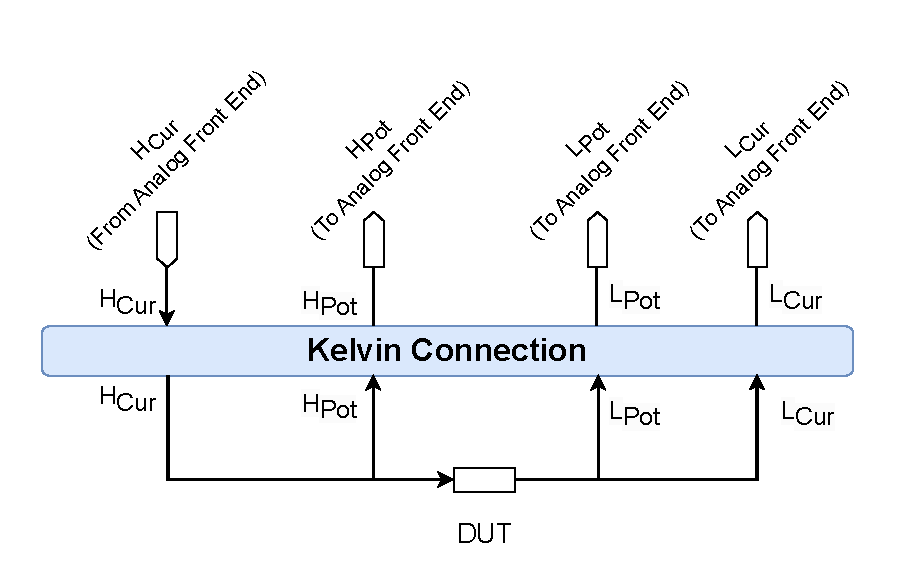
\includegraphics[clip, trim=18 0 18 0,width=0.70\textwidth]{Sections/6_SystemArchitecture/Figures/Kelvin Connection.pdf}
    \caption{A Kelvin connection (4-wire). The $H_{CUR}$ (\textit{high current}), and $L_{CUR}$ signals are the high current running through the DUT. This current is sampled across the range resistors in the analog front end. $H_{pot}$ (\textit{high potential}) and $L_{pot}$.}
    \label{fig_6_2_KelvinConnection}
\end{figure}

The kelvin connection is a standard interface used by many commercial instruments. It must conform to a common physical layout in order to accept common capacitance and inductance reference standards. This will be shown in the module specifications and interface.


